\subsection{Binary Exactness and Frontend Loss}\label{sec:utility_results}

On the frozen CelebA roots, all 1,310,720 tested re-keyed bits and 1,310,720 protected probe/gallery scores agree with their reference across 20 epochs. This is exactness relative to the binary frontend.

On the fixed CelebA gallery/probe images, float Rank-1/Rank-5 are 0.8691/0.9473, versus binary 0.8516/0.9375. Twenty paired splits on the portability cohort give mean float/binary Rank-1 0.8762/0.8515. The paired binary-minus-float difference is -2.471 percentage points (identity-bootstrap 95\% interval [-3.281, -1.729]). Image-level reproduction checks for both cohorts are documented in the supplement.

On LFW, native FaceNet sign binarization loses 0.420 percentage points at 128 and 1.641 points at 4096 (paired 95\% interval at 4096: $[-2.480,-0.850]$ points). Masking adds zero binary-domain score error; it does not recover frontend loss.

\begin{table}[t]
\caption{Paired LFW Rank-1 percentages over 20 frozen assignments; the same 128 query identities at each size. Both fixed centered projections are shown, without selecting a seed.}
\label{tab:v3frontend}\centering\small
\setlength{\tabcolsep}{3pt}
\begin{tabular}{llrr}
\toprule
Frontend & Bits & $N=128$ & $N=4096$ \\
\midrule
FaceNet float & 512D & 98.91 & 95.31 \\
FaceNet sign & 512 & 98.49 & 93.67 \\
SFace float & 128D & 98.89 & 98.60 \\
SFace sign & 128 & 96.60 & 91.04 \\
SFace RP seed 1 & 512 & 98.54 & 97.29 \\
SFace RP seed 2 & 512 & 98.53 & 96.89 \\
\bottomrule
\end{tabular}
\end{table}

\begin{figure*}[t]\centering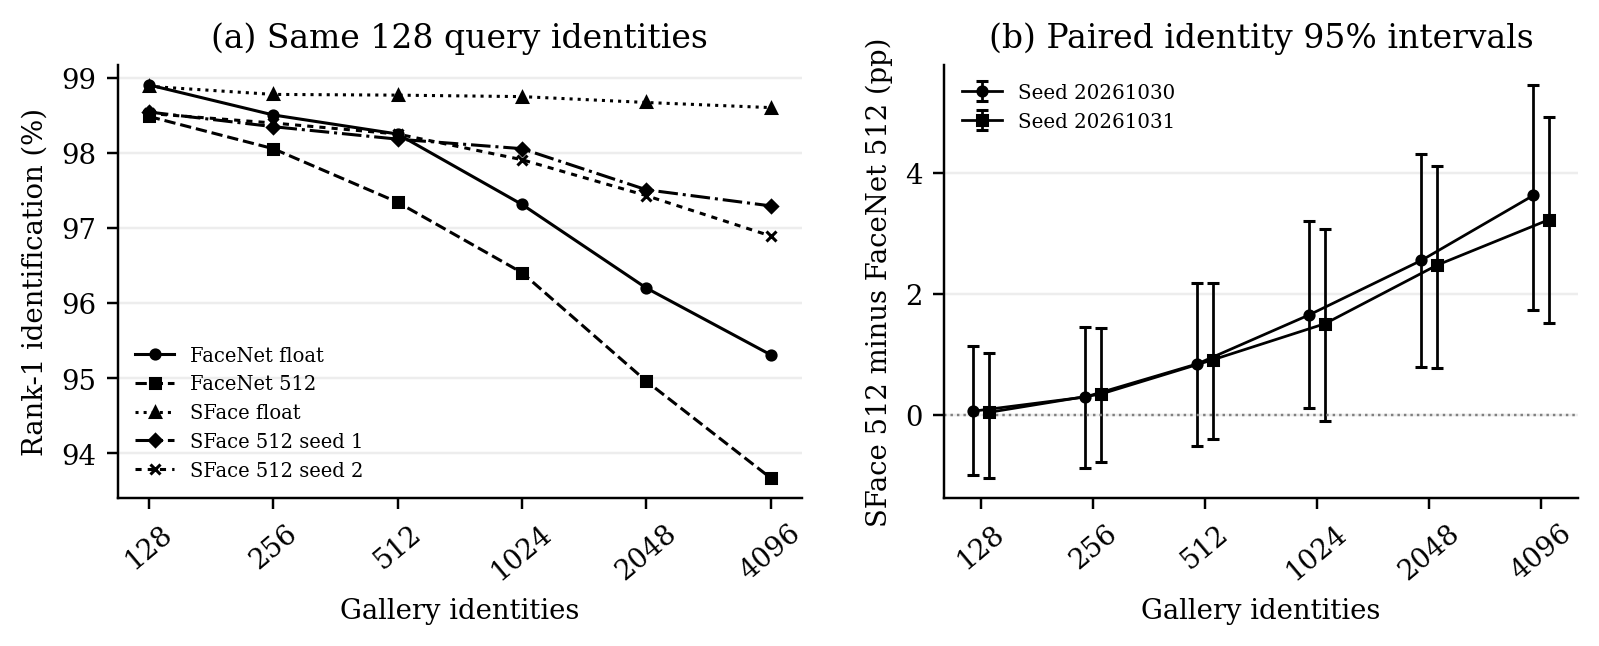
\includegraphics[width=\textwidth]{figures/frontend_scale_v3.png}\caption{Paired utility with the same 128 query identities across nested galleries. Both fixed SFace 512-bit projection seeds are retained; the right panel compares them with native FaceNet 512-bit signs. Intervals resample identities after averaging 20 repeated assignments and are conditional on the frozen gallery/calibration pools.}\label{fig:paired_scale}\end{figure*}

At 4096 entries, centered SFace 512 projections give 97.295\% and 96.895\% Rank-1 for seeds 20261030 and 20261031, versus 93.672\% for FaceNet 512 signs. Paired gains are 3.623 points (95\% interval $[1.729,5.449]$) and 3.223 points ($[1.514,4.922]$). The two code instances are reported separately; their mean is not an ensemble prediction. The same frozen transforms give 89.951\%/90.381\% on the fixed CelebA cohort and 91.846\%/91.768\% on the portability cohort, compared with 86.055\%/85.146\% FaceNet 512 baselines respectively. Model, alignment and coding change together. No unseen-identity or isolated-hash improvement is inferred.

\begin{table}[t]
\caption{Open-set results at 4096 gallery entries. Same 512 calibration and 512 unknown identities; actual test FPIR and DIR percentages, not nominal operating points.}
\label{tab:v3open}\centering\small
\setlength{\tabcolsep}{3pt}
\begin{tabular}{llrr}
\toprule
Frontend & Rule & FPIR & DIR \\
\midrule
FaceNet 512 & Emp. & 1.172 & 59.12 \\
FaceNet 512 & Cons. & 0.391 & 46.33 \\
SFace 512 seed 1 & Emp. & 3.252 & 91.42 \\
SFace 512 seed 1 & Cons. & 1.758 & 85.44 \\
SFace 512 seed 2 & Emp. & 2.363 & 89.92 \\
SFace 512 seed 2 & Cons. & 1.562 & 86.10 \\
\bottomrule
\end{tabular}
\end{table}

Actual test FPIR is reported beside DIR. The conservative rule gives 1.758\%/1.563\% FPIR and 85.44\%/86.10\% DIR for the two SFace 512 seeds, compared with 0.391\% and 46.33\% for FaceNet 512. This is not an equal-FPIR comparison. Results for a separate 32-identity frequent-image pilot and all less favorable preprocessing variants are reported in the supplement/artifact. We do not claim reliable performance at FPIR $10^{-3}$ from 512 unknowns.

\subsection{Retrieval and Complete Private Query}\label{sec:query_results}

\begin{table}[t]
\caption{Unbounded candidate union on one frozen LFW split. Capacity-failing rows are diagnostics, not admitted secure indices.}
\label{tab:index}\centering\small
\setlength{\tabcolsep}{3pt}
\begin{tabular}{rrrrrr}
\toprule
Gallery & $w$ & Recall & Agreement & Fraction & Fallback \\
\midrule
128 & 4 & 1.0000 & 1.0000 & 0.9980 & 0.0566 \\
128 & 8 & 0.9941 & 0.9980 & 0.3049 & 0.9570 \\
4096 & 4 & 1.0000 & 1.0000 & 0.9980 & 0.1758 \\
4096 & 8 & 0.9941 & 0.9980 & 0.2893 & 0.9570 \\
\bottomrule
\end{tabular}
\end{table}

Four-bit buckets retrieve almost the whole gallery. At 4096 entries, eight-bit buckets retrieve about 29\%, but require certified fallback on 95.70\% of probes. Their public capacity is 72 versus 138 required, so enrollment rejects or reconfigures. Certified selection agrees with exhaustive decisions for every evaluated probe. Both SFace 512 codes also have near-one four-bit candidate fractions; no pruning speedup follows.

\begin{table}[t]
\caption{Full $N=128$ query from the same persisted state with private client input/output: five balanced measured trials. Candidate and exhaustive winners agree.}
\label{tab:v3privatequery}\centering\small
\setlength{\tabcolsep}{3pt}
\begin{tabular}{lrr}
\toprule
Method & Seconds & Global MB \\
\midrule
Full scan & $5.99\pm1.29$ & 123.77 \\
Fused blocks & $5.93\pm0.62$ & 143.91 \\
Polynomial index & $25.10\pm8.14$ & 792.37 \\
\bottomrule
\end{tabular}
\end{table}

The exact polynomial index operator is faster than repeated full-field equality, but still adds work to the full matcher. Reusing already computed mismatch bits produces the same candidate flags without reading the index; full scan needs no candidate construction. The complete controls return the same identity/reject result from the same persisted state. Independent candidate-bit oracles cover mixed/no/all sets and a three-row gallery, preventing exhaustive fallback from concealing retrieval defects.

\subsection{State Integrity and Linkage Diagnostics}\label{sec:integrity_results}

In the materialized reference, all eight injected faults are rejected, the previous logical state is retained, and the post-rejection query agrees with the independent oracle. Primitive tests also agree at full field width. In the SHAKE simulation, direct linkage AUC is 0.4948, direct assignment 0.0066 and relational assignment 0.0082, against chance 1/128 for assignment; the global-mask relational control is 1.0000. These are attack-specific observations, not an exposed-key or general irreversibility proof.

\begin{table}[t]
\caption{Joint-invariant witnesses. A/R: accept/reject; --: unmeasured. Bind and Rel. enable only template binding or index relation. The coupled mutation changes a root bit and its bucket occurrence together. Wrong-state acceptances occur in the reduced checkers.}
\label{tab:joint_ablation}\centering\small
\setlength{\tabcolsep}{3pt}
\begin{tabular}{r l c c c}
\toprule $N/d$ & Mutation & Bind & Rel. & Both \\
\midrule
4/64 & None & A & A & A \\
4/64 & Omit slot & A & R & R \\
4/64 & Root+bucket & R & A & R \\
8/512 & Root+bucket & -- & A & R \\
\bottomrule\end{tabular}\end{table}

A coupled mutation changes a root bit and moves its index occurrence into the corresponding new bucket. Relation-only checking accepts the wrong enrolled root at both tested sizes; full binding rejects it. Template-only checking misses an omitted occurrence. The virtual view excludes a stale-handle no-op from its rejection count. These witnesses concern application invariants under passive MPC, not malicious-protocol soundness.

\subsection{Complete Renewal and Simpler Controls}\label{sec:cost_results}

\begin{table}[t]
\caption{Actual persisted-share rekeying: five alternating measured trials, mean and sample SD. All five parties are local.}
\label{tab:v3persisted}\centering\small
\setlength{\tabcolsep}{3pt}
\begin{tabular}{rlrr}
\toprule
$N$ & Representation & Seconds & Global MB \\
\midrule
128 & Materialized & $27.81\pm0.94$ & 2710.0 \\
128 & Virtual & $12.80\pm1.44$ & 590.0 \\
\bottomrule
\end{tabular}
\end{table}

\begin{table}[t]
\caption{Larger real LFW galleries, FaceNet 512-bit roots: three measured cold-input trials per completed cell. VM time and global traffic; initialization fixture is a trusted input owner.}
\label{tab:v3scale}\centering\small
\setlength{\tabcolsep}{3pt}
\begin{tabular}{rllrr}
\toprule
$N$ & Operation & View & Seconds & MB \\
\midrule
512 & Rekey & Materialized & $140.19\pm17.35$ & 9783.1 \\
512 & Rekey & Virtual & $67.61\pm16.33$ & 2576.9 \\
512 & Query & Materialized & $28.59\pm2.11$ & 490.0 \\
512 & Query & Virtual & $29.23\pm3.67$ & 503.3 \\
1024 & Rekey & Materialized & $202.81\pm40.77$ & 19389.7 \\
1024 & Rekey & Virtual & $113.15\pm35.64$ & 5402.1 \\
1024 & Query & Materialized & $26.80\pm2.49$ & 1019.0 \\
1024 & Query & Virtual & $26.23\pm1.58$ & 1045.6 \\
\bottomrule
\end{tabular}
\end{table}

The persisted-share comparison includes loading, old/new masks, full relation and binding checks, selection, complete-row shuffle, every-field share refresh and writes. Its paired materialized control is 27.81 s at 128; the input-inclusive reference is measured separately. Larger-gallery cold-input runs use real LFW roots but a trusted protected-state input owner. These interfaces are not pooled. Timing, traffic, rounds and largest-party RSS are recorded; non-monotonic cross-size timings and variability do not establish a latency scaling law.

\begin{table}[t]
\caption{Conventional-cipher control, five measured rekeys. Both ciphers implement the same high-level invariant/check/maintenance contract in arithmetic Shamir MPC.}
\label{tab:v3cipher}\centering\small
\setlength{\tabcolsep}{3pt}
\begin{tabular}{rllrr}
\toprule
$N$ & View & Cipher & Seconds & MB \\
\midrule
2 & Materialized & AES-CTR & $3.20\pm0.59$ & 177.2 \\
2 & Materialized & MiMC & $4.17\pm0.61$ & 118.5 \\
8 & Virtual & AES-CTR & $4.45\pm0.46$ & 273.8 \\
8 & Virtual & MiMC & $4.31\pm0.76$ & 47.4 \\
32 & Virtual & AES-CTR & $10.97\pm1.62$ & 1053.2 \\
32 & Virtual & MiMC & $6.85\pm2.59$ & 148.8 \\
\bottomrule
\end{tabular}
\end{table}

AES-CTR passes three independent/MPC known-answer vectors and the same state checks. AES is faster in the smallest materialized case; the 32-record virtual comparison favors MiMC in this arithmetic backend. Conventional encryption supports the useful lifecycle contract. Shared raw roots already protect below-threshold party views and remove mask costs. Complete matched raw-root and full-width compact-sort controls, phase breakdowns and timing ranges are reported in the supplement. The quadratic pointer join is not the main transition comparator.

Task-local stream-delay tests separately examine added RTT 0/1/20/50 ms with echo calibration. Results are reported by tested size; all parties remain on one host, and the small 64-bit rekey is not extrapolated to 512-bit deployment. Relay queueing and controller CPU are disclosed with the complete measurements.
